% Chapter Template

\chapter{Ensayos y resultados} % Main chapter title

\label{Chapter4} % Change X to a consecutive number; for referencing this chapter elsewhere, use \ref{ChapterX}

%----------------------------------------------------------------------------------------
%	SECTION 1
%----------------------------------------------------------------------------------------
\section{Aplicación}

La aplicación se encarga de ayudar a los operadores durante la fabricación por lotes de un producto determinado. Durante los procedimientos \textit{batch} se utilizan el mismo conjunto de máquinas para la fabricación de distintos productos. Por lo tanto, las tareas de los operadores varían en las distintas partes del proceso dependiendo del producto que se esté fabricando. 

Una etapa clave en la fabricación del producto, es el agregado de aditivos en la mezcla. La aplicación desarrollada se encarga de evitar que el operador falle a la hora de seleccionar y dosificar el aditivo requerido. La aplicación comienza con la imagen que se muestra en la figura \ref{fig:i2}.

\begin{figure}[htpb]
	\centering
	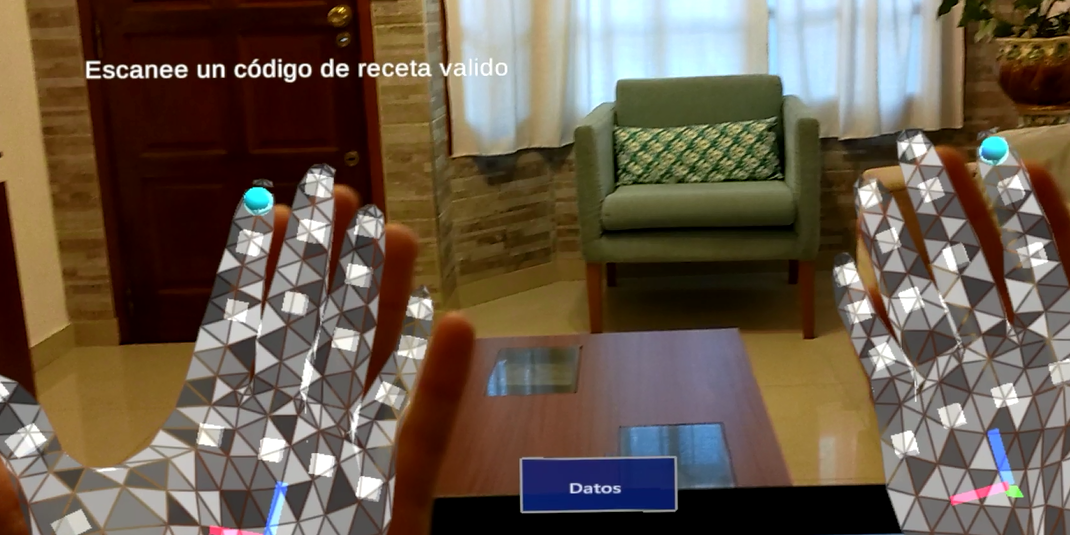
\includegraphics[scale=.5]{./Figures/i2.PNG}
	\caption{Pantalla inicial\protect\footnotemark.}
	\label{fig:i2}
\end{figure}

En este punto se aguarda la lectura del codigo QR correspondiente a la receta a producir. Las recetas son el conjunto de parámetros que involucran un lote de producción. En ellas se puede encontrar el listado de aditivos, la cantidades requeridas, los códigos de los distintos productos tiempos de mezclado y demás parámetros necesarios para la producción. Si el operador lee un código de receta para el cual el sistema de control no fue configurado a producir en ese momento, se indicará un error como muestra la figura \ref{fig:i3}.

\begin{figure}[!htpb]
	\centering
	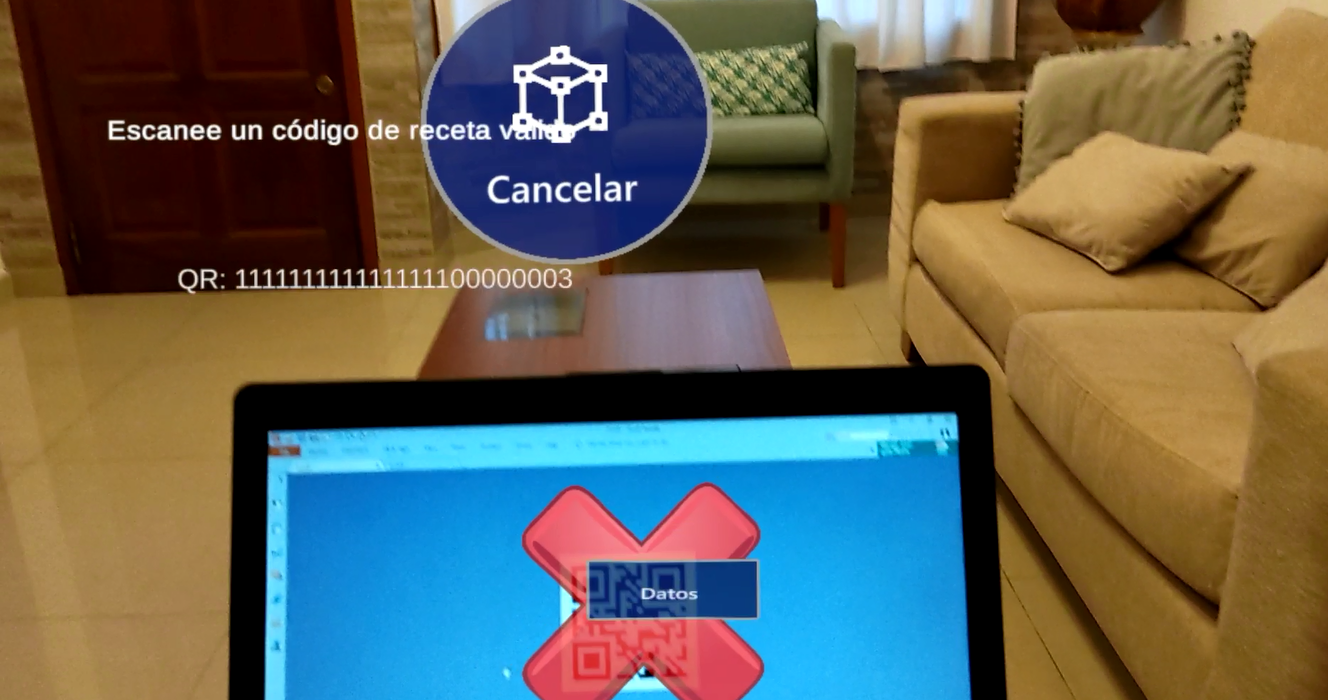
\includegraphics[scale=.3]{./Figures/i3.PNG}
	\caption{Código erróneo\protect\footnotemark.}
	\label{fig:i3}
\end{figure}

Para poder avanzar, es necesario que se lea el código de la receta correcta, como se muestra en la figura \ref{fig:i4}.

\begin{figure}[!htpb]
	\centering
	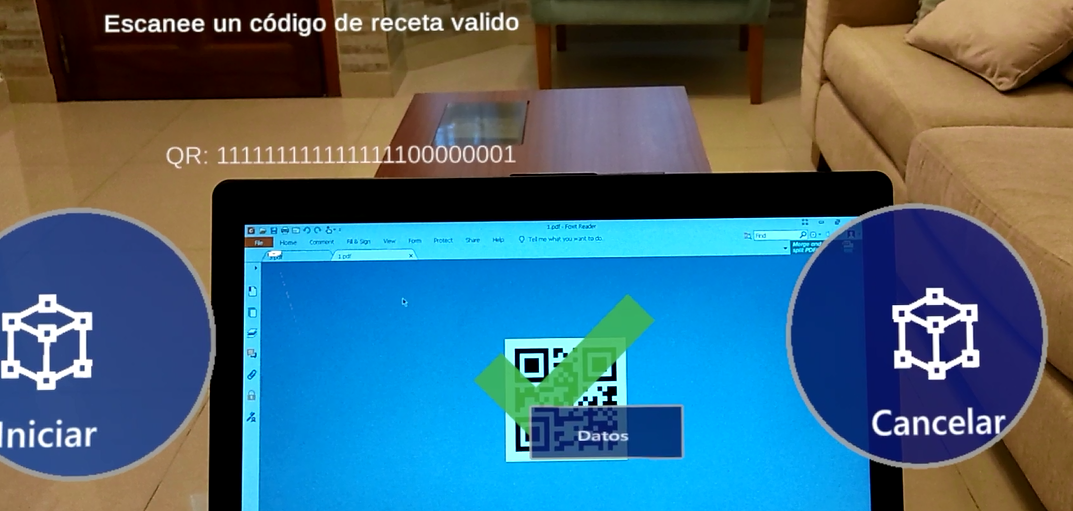
\includegraphics[scale=.4]{./Figures/i4.PNG}
	\caption{Código correcto\protect\footnotemark.}
	\label{fig:i4}
\end{figure}

En éste punto el operador acepta la receta y la interfaz mostrará la imagen que se presenta en la figura \ref{fig:i6}.

\begin{figure}[!htpb]
	\centering
	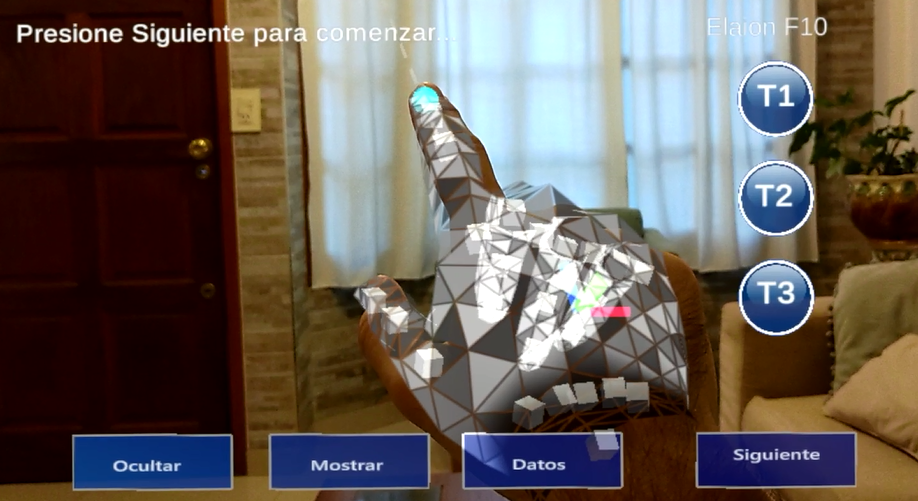
\includegraphics[scale=.4]{./Figures/i6.PNG}
	\caption{Inicio de receta\protect\footnotemark.}
	\label{fig:i6}
\end{figure}

En el margen derecho se pueden ver tres círculos azules, los cuales representan tres tareas del operador a lo largo de la receta de producción. En la parte superior del listado de tareas se puede leer el producto que se fabricará en esta receta. En el lado izquierdo superior se puede ver una leyenda que irá actualizándose para guiar al operador. En la parte inferior se encuentran cuatro botones con las siguientes funcionalidades:

\begin{itemize}
\item Ocultar: permite simplificar la vista holográfica, reduciendo la información proyectada en el Hololens 2.
\item Mostrar: restablece la información holográfica oculta.
\item Datos: muestra los datos del código QR leído.
\item Siguiente: se utiliza para avanzar a la siguiente etapa.
\end{itemize}

Según lo indicado en pantalla el operador deberá pulsar ``Siguiente'' para iniciar el procedimiento como se muestra en la figura \ref{fig:i6}. En ese momento la instrucción se modificará, solicitándole que vierta en el tanque de producción el producto A. Esto se ilustra en la imagen de la figura \ref{fig:i7}.

\begin{figure}[!htpb]
	\centering
	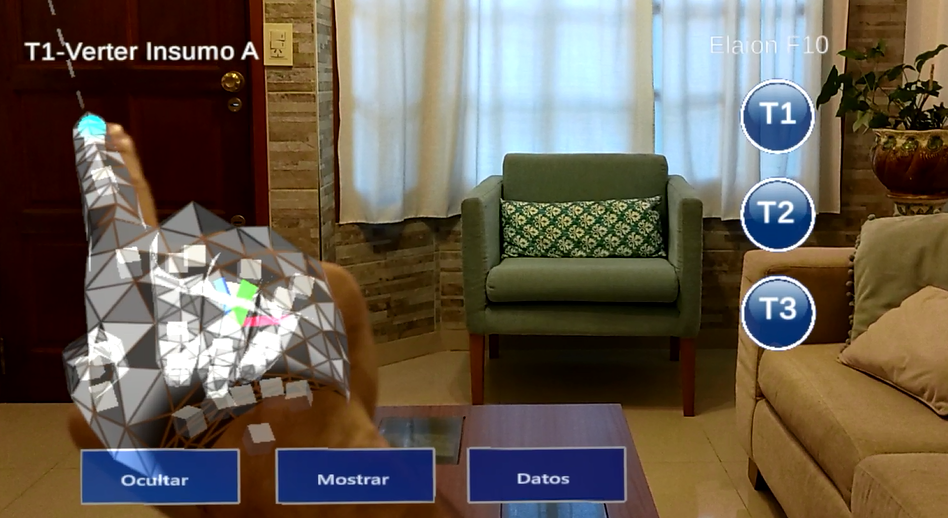
\includegraphics[scale=.4]{./Figures/i7.PNG}
	\caption{Selección insumo\protect\footnotemark.}
	\label{fig:i7}
\end{figure}

El operador deberá localizar las bolsas de éste producto y leerá con el Hololens 2 el código QR de la misma. En ese momento el conjunto de datos se actualizará como se ilustra en la imagen de la figura \ref{fig:i8}.

\begin{figure}[!htpb]
	\centering
	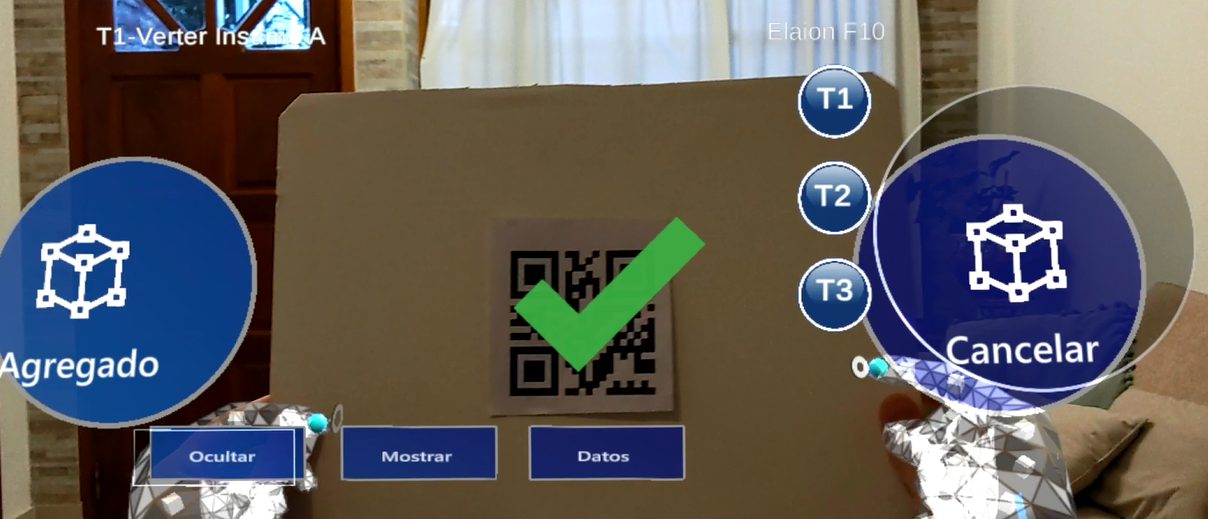
\includegraphics[scale=.4]{./Figures/i8.PNG}
	\caption{Insumo correcto\protect\footnotemark.}
	\label{fig:i8}
\end{figure}

Si el producto es correcto se mostrará un tilde verde, de lo contrario se mostrará una cruz roja como en la figura \ref{fig:i3}. El operador pulsara ``Agregado'' y luego deberá verter las cantidades indicadas del producto en el tanque de producción. En el centro izquierdo de la imagen, se pueden ver los datos que hacen referencia al aditivo que se usará en la receta. Como se ilustra en la imagen de la figura \ref{fig:i9}.

\begin{figure}[!htpb]
	\centering
	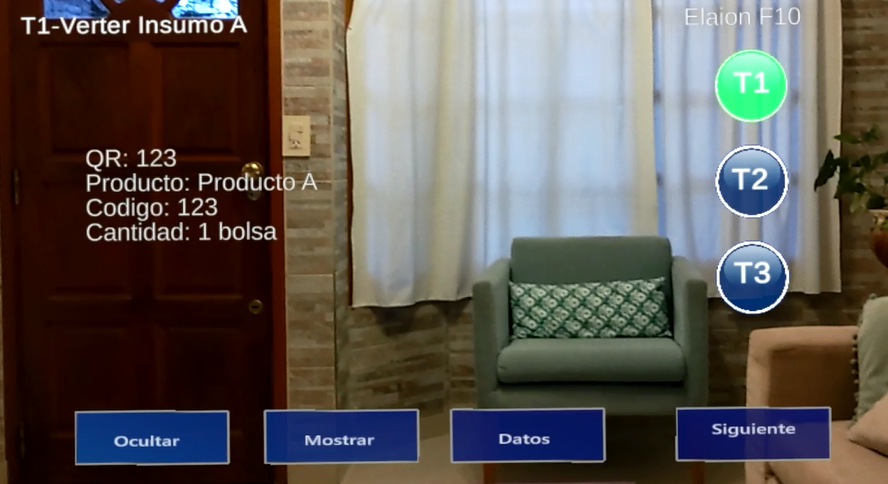
\includegraphics[scale=.5]{./Figures/i9.PNG}
	\caption{Producto elegido\protect\footnotemark.}
	\label{fig:i9}
\end{figure}

Se muestran los siguientes datos:

\begin{itemize}
\item QR: código QR leído por el Hololens 2.
\item Producto: nombre del producto leído. 
\item Código: código del producto leído.
\item Cantidad: cantidad necesaria del producto en la receta.
\end{itemize}

Luego el operador pulsara ``Siguiente'' y se actualizará la información con una nueva instrucción como se ilustra en la figura \ref{fig:i11}.

\begin{figure}[!htpb]
	\centering
	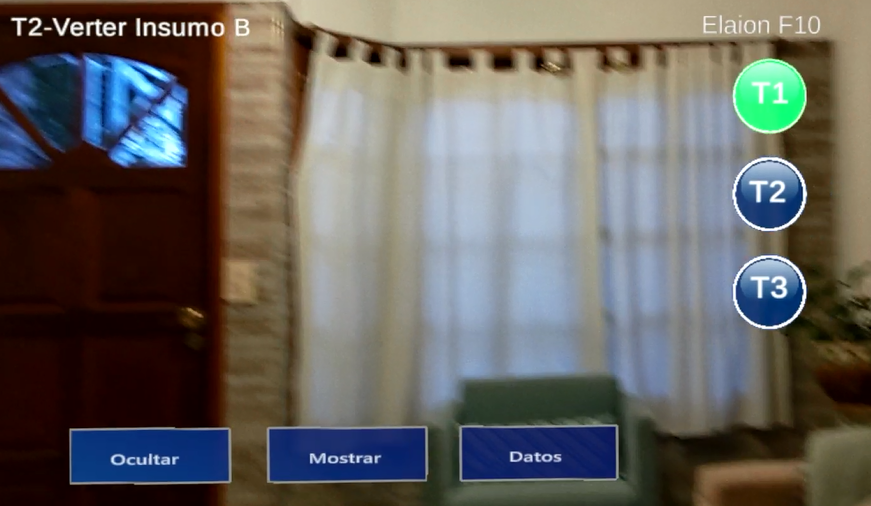
\includegraphics[scale=.5]{./Figures/i11.PNG}
	\caption{Selección de producto\protect\footnotemark.}
	\label{fig:i11}
\end{figure}

El procedimiento se repetirá para el total de las tareas de la receta y a medida que las tareas se completen se pintaran de color verde. Luego de la última operación, se mostrará la leyenda ``Procedimiento terminado 3/3'', como se ilustra en la imagen de la figura \ref{fig:i18} indicándole al operador que puede cerrar la aplicación.

\begin{figure}[!htpb]
	\centering
	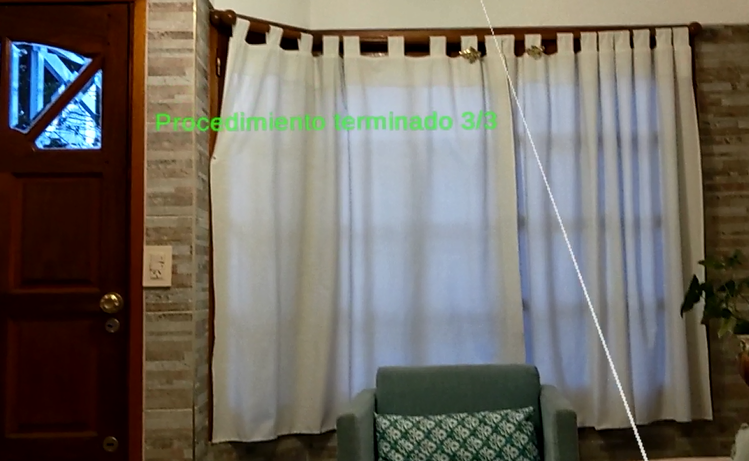
\includegraphics[scale=.5]{./Figures/i18.PNG}
	\caption{Fin de la aplicación\protect\footnotemark.}
	\label{fig:i18}
\end{figure} 

Los comandos al sistema de control son enviados luego de que el producto correcto fue leído y el operador avanza al siguiente paso de la receta, garantizando que se cumplió la tarea asignada. Si el producto erróneo es leído, el operador no tiene habilitado el paso siguiente, por lo tanto queda retenido en esa etapa. Además, las recetas válidas son sólo aquellas en las que el sistema de control aguarda operaciones manuales, de esta manera se asegura que no puedan mezclarse otras recetas con la receta activa.

\section{Evaluación de las interfaces}
\label{sec:pruebasHW}

A continuación se puede ver algunas mediciones de tiempos de respuesta de las interfaces principales. Para la medición Hololens 2 - API, se utilizó la opción \textit{debug} del Hololens 2 para identificar el \textit{timestamp} del comando emitido al clickear ``Siguiente'' en la interfaz. Además se utilizó la API para loguear el \textit{timestamp} en el que se recibe la consulta web.\\

Para la medición API - server OPC, también se utilizó la API para loguear el \textit{timestamp} en el que se recibe la consulta web. Y se utilizó el servicio OPC para loguear el momento en el que la variable OPC es actualizada. Para un promedio de 10 mediciones consecutivas, los resultados pueden verse en la tabla \ref{tab:interfaces}.

\begin{table}[htpb]
	\centering
	\caption[Tiempos de respuesta]{Tiempos de respuesta promedio}
	\scalebox{0.9}{
	\begin{tabular}{l c c}    
		\toprule
		\textbf{Interfaz} 	 & \textbf{Tiempo}  \\
		\midrule
		Hololens 2 - API				&  >340ms \\		
		API - server OPC	 		&  >320ms \\
		\bottomrule
		\hline
	\end{tabular}}
	\label{tab:interfaces}
\end{table}

Dado que la aplicación se comunica a través de mensajes del tipo JSON y la cantidad de información enviada es reducida, los tiempos de respuesta son realmente bajos y no representan un problema para la implementación. Se puede ver que el tiempo de respuesta de toda la cadena de comunicación es inferior al segundo. Este trabajo se realizó utilizando servidores \textit{cloud} pero bien podrían ser locales. Llegado el caso, si los tiempos representan una pérdida de fluidez en la aplicación, la migración no requeriría mayores esfuerzos. 

\section{Devoluciones del cliente}
Las presentaciones realizadas a usuarios industriales resaltaron las fortalezas de la tecnología. Se presento interés en desarrollar aplicaciones orientadas al mantenimiento de maquinas. Estableciendo una serie de pasos que el operador debe realizar periódicamente para prolongar la vida útil de la maquina. También se menciono su aplicación en el entrenamiento para el uso de las maquinas. Donde el operador pueda ensayar en primer instancia, sobre una replica holográfica de la maquina las distintas configuraciones de operación. Y en segunda instancia, asistido por instrucciones holográficas sobre la maquina real. Por ultimo, se identificaron operatorias en planta donde el Hololens 2 podría reducir los tiempos de operación. Ahorrándole al operador la necesidad de consultar los sistemas de producción en busca de ordenes de trabajo, identificaciones de productos o estado de distintos equipos en el sistema de control.